\documentclass[a4paper,twoside,11pt]{article}
\usepackage[utf8]{inputenc}
\usepackage[english]{babel}
\usepackage{subcaption}
\usepackage{graphicx}
\usepackage{url}
\usepackage{titlesec}
\usepackage{tikz}
\usetikzlibrary{er}
\usepackage[justification=centering]{caption}


% Redefinição das margens das páginas
\setlength{\textheight}{24.00cm}
\setlength{\textwidth}{15.50cm}
\setlength{\topmargin}{0.35cm}
\setlength{\headheight}{0cm}
\setlength{\headsep}{0cm}
\setlength{\oddsidemargin}{0.25cm}
\setlength{\evensidemargin}{0.25cm}
\setlength{\parindent}{0pt}

\begin{document}

\vspace{-15mm}
\begin{figure}[h]
\begin{center}
\resizebox{80mm}{!}{
\includegraphics{images/logoISEL.png}}
\end{center}
\end{figure}
\vspace{-8mm}

% Title Section
\begin{center}
    \LARGE \textbf{LiftDrop} \\ % Bold title
    \LARGE Mobile App for Deliveries \\ % Subtitle in normal weight
    \vspace{8mm}
    \large Gonçalo Morais, n.º 49502, e-mail: a49502@alunos.isel.pt, tel.: 927468061 \\
    \vspace{1mm}
    \large João Ramos, n.º 49424, e-mail: a49424@alunos.isel.pt, tel.: 919222551 \\
    \vspace{5mm}
    \large \textbf{Orientador:} Miguel Gamboa, e-mail: miguel.gamboa@isel.pt \\
    \vspace{3mm}
    \large \textbf{Co-Orientador:} Diogo Silva, e-mail: diogo.silva@lyzer.tech \\
    \vspace{5mm}
    \textbf{March of 2025}
\end{center}

\section {Resume} 

The rise of the \textbf{gig economy} has transformed various industries, particularly the food and package delivery sector. This economic model relies on flexible short-term work arrangements, often facilitated through digital platforms. Companies such as Uber Eats, Glovo, and Bolt Food have leveraged this framework to revolutionize urban logistics, enabling customers to order food and services on demand while offering couriers independent work opportunities.

\vspace{5mm}

Although these platforms prioritize customer convenience, they also present significant challenges for couriers. High commission fees, lack of job stability, and inefficiencies in delivery logistics create an imbalance between platform profitability and worker sustainability. In addition, customers often experience delays and inconsistent service quality.

\vspace{5mm}

To address these challenges, LiftDrop proposes a new approach to the gig economy by offering a more fair, efficient, and transparent delivery solution. This mobile app aims to improve courier conditions while enhancing the customer experience through optimized delivery processes and fairer economic policies.

\section{Introduction}
The gig economy has revolutionized delivery services, but existing platforms often prioritize customer convenience over courier well-being. LiftDrop addresses this gap by proposing a fairer, more efficient mobile app for deliveries.

\vspace{3mm}

\textbf{Key Goals:}

\begin{itemize}
    \item Optimize order assignment using real-time data (proximity, traffic, fairness)
    \item Enhance courier safety with neighborhood ratings and alerts
    \item Streamline operations via a scalable Android app backed by two APIs:
    \begin{itemize}
        \item \textbf{Courier API} (order management, real-time updates via SSE)
        \item \textbf{Client Simulation API} (mock orders for testing)
    \end{itemize}
\end{itemize}

\vspace{5mm}

The diagram below provides a high-level overview of LiftDrop's architecture:

\vspace{3mm}

\begin{figure}[h]
    \centering
    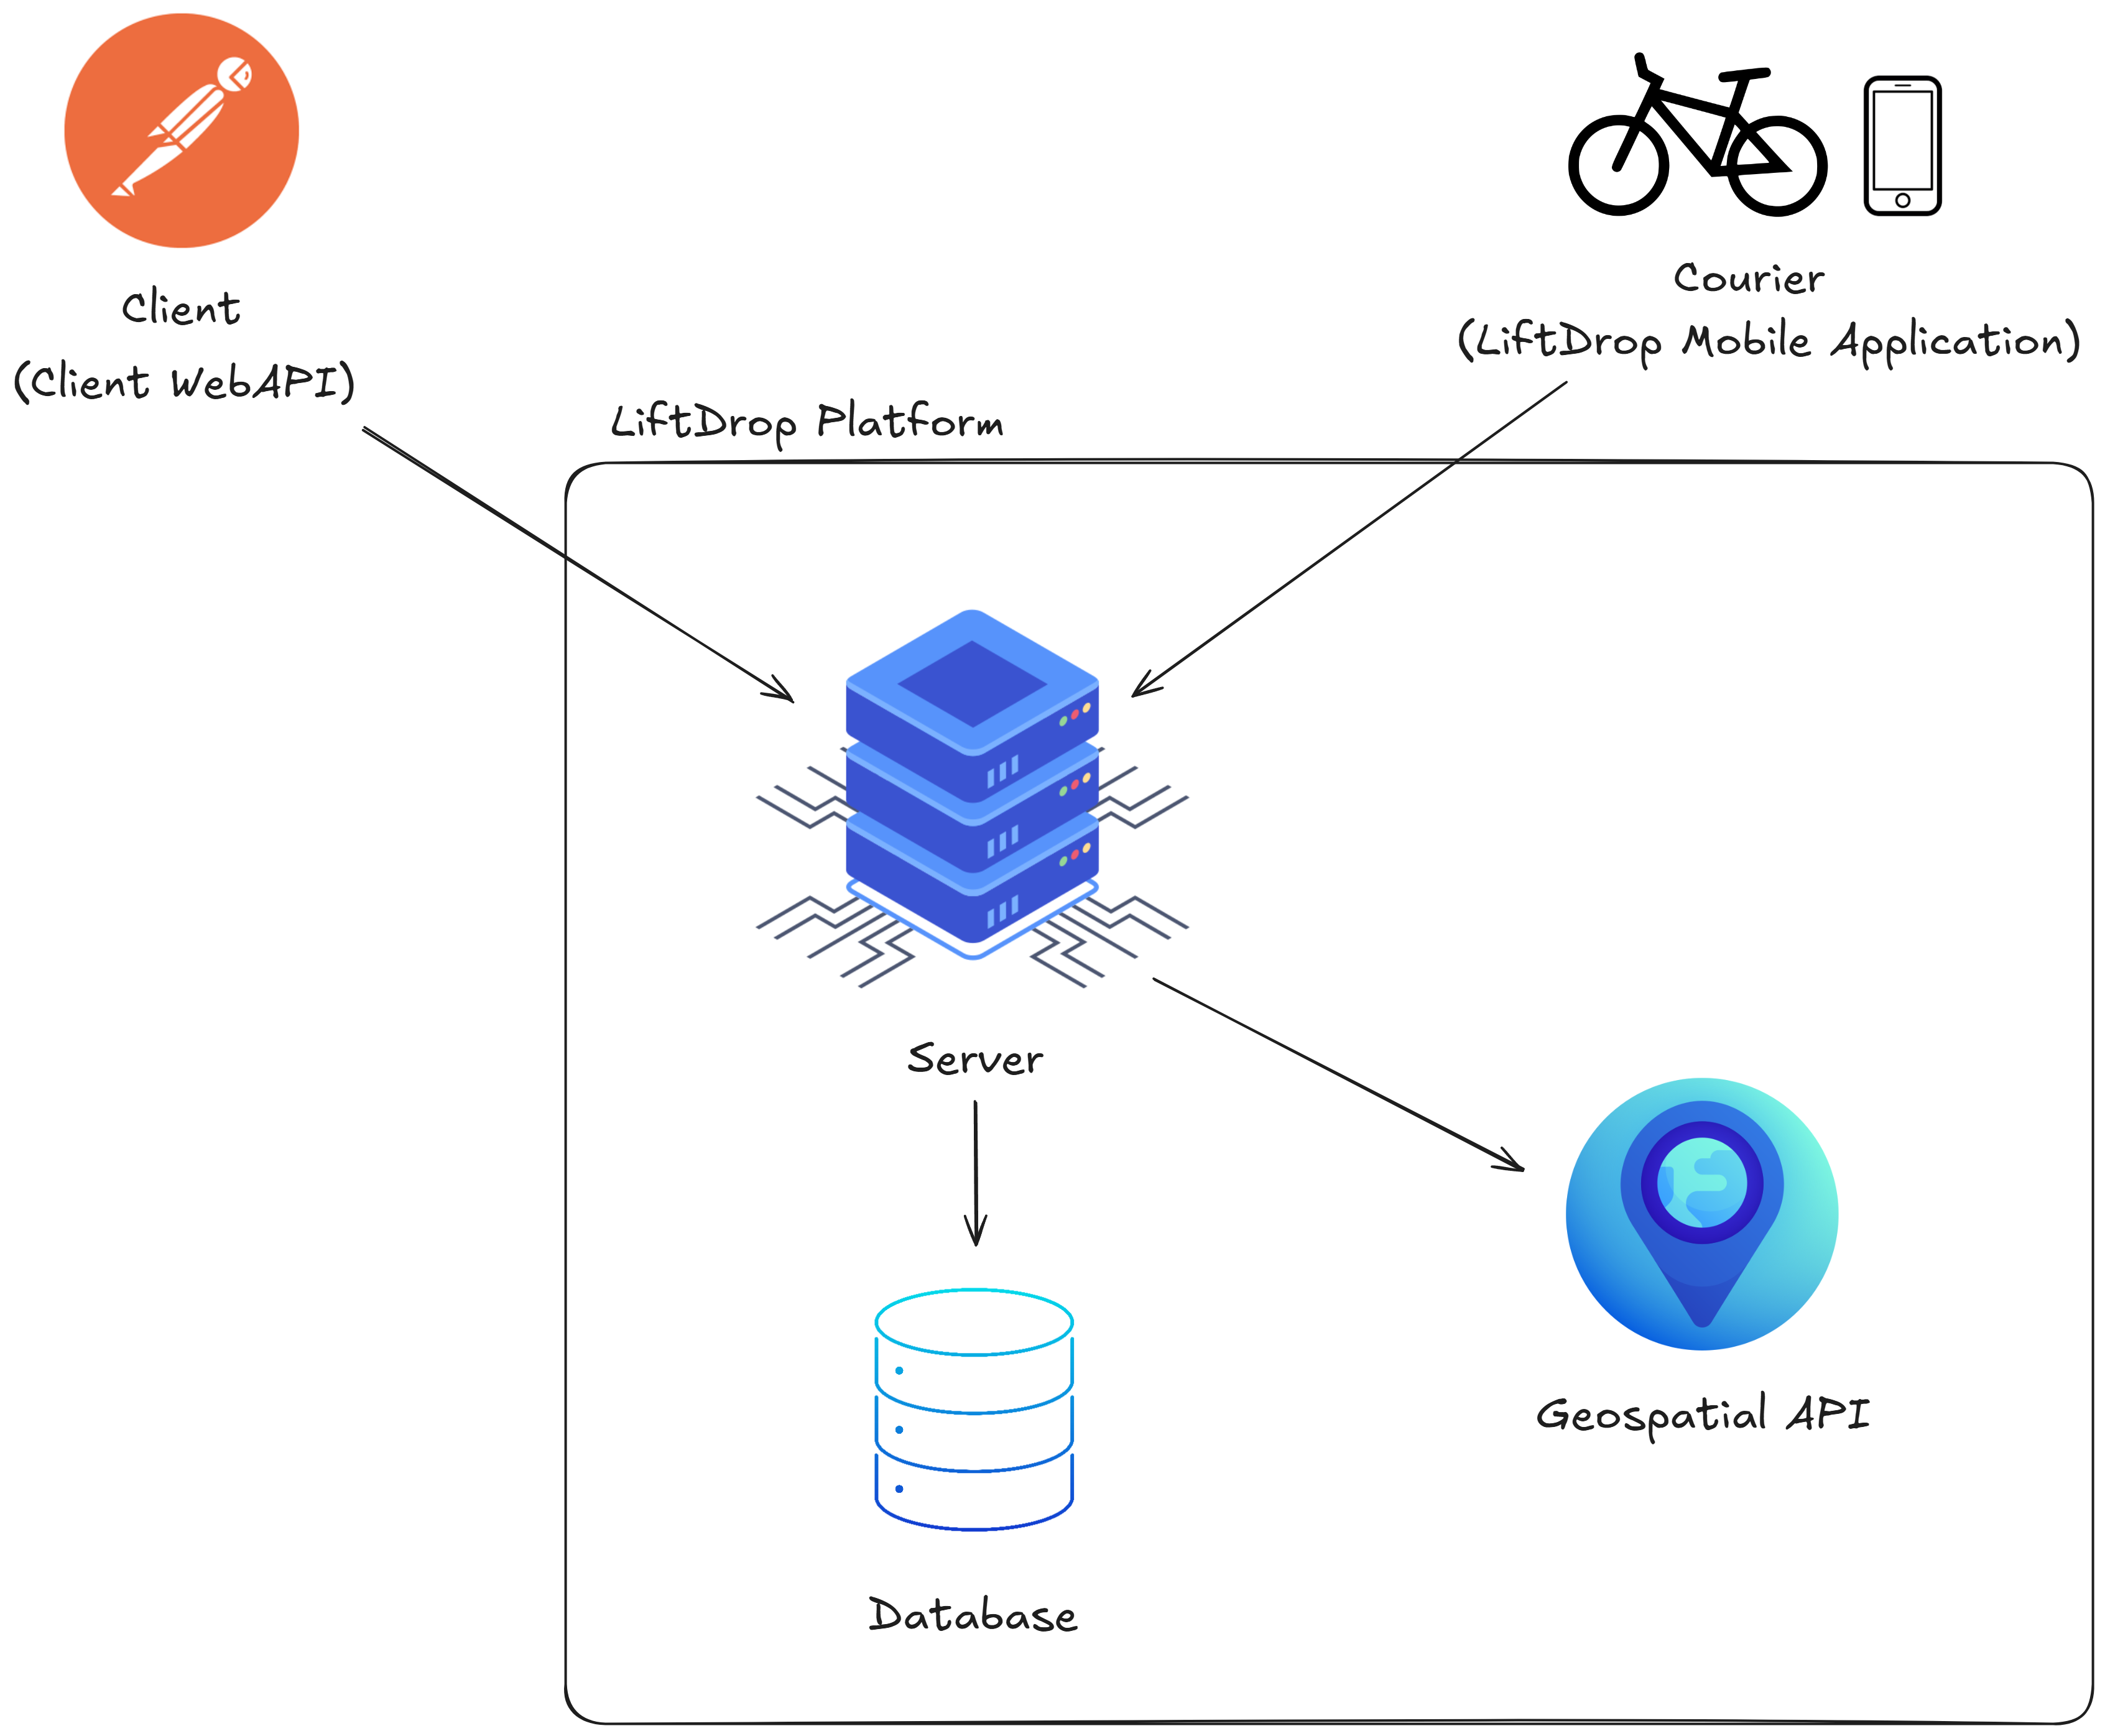
\includegraphics[width=0.8\textwidth]{images/LiftDrop_High_level_view.png}
    \caption{High-level overview of the platform, showing interaction between clients, server, database and external APIs (Google Maps).}
    \label{fig:high_level}
\end{figure}


\section{Scope}

\subsection{Scope Features}  

\subsubsection{Client Features}  
\begin{itemize}
    \item Place an order by selecting a restaurant and desired items.
    \item Track the order status and receive estimated time of arrival.
\end{itemize}

\subsubsection{Courier Features}  
\begin{itemize}
    \item Accept or decline incoming orders.
    \item Set availability by starting or stopping waiting status.
    \item Update order status after acceptance.
    \item Cancel an order if needed.
    \item Confirm delivery upon completion.
\end{itemize}

\subsubsection{User Features}  
\begin{itemize}
    \item Register as either a client or a courier.
    \item Clients provide personal and contact information during registration.
    \item Couriers specify their means of transportation upon registration.
\end{itemize}
  

\subsection{Real-Time Data Handling and Order Assignment}  

Developing a mobile application focused on delivery presents challenges, particularly in real-time data handling and order assignment. Since multiple couriers interact with the platform simultaneously, the system must manage updates effectively while ensuring a smooth user experience. After research and consideration, we identified three primary approaches to handling real-time updates and concurrency:

\begin{itemize}
    \item \textbf{Polling-based Request-Response Model} – The client periodically requests updates from the server. While simple to implement, this approach results in unnecessary network requests, increased server load, and delayed updates.
    \item \textbf{WebSockets} – A bidirectional communication protocol that allows both the client and server to send messages dynamically. While WebSockets are ideal for interactive, two-way communication (e.g., chat applications), SSE offers a simpler and more reliable approach for our needs, focusing on server-driven updates.
    \item \textbf{Event-Driven Server-Sent Events (SSE)} – The server pushes updates to clients as they occur, enabling real-time communication without the inefficiencies of constant polling. This is well-suited for unidirectional data flow (server-to-client updates).
\end{itemize}

Given the requirements of this project, we chose \textbf{SSE} as the preferred method for real-time updates due to its simplicity, maintainability, and efficient handling of one-way event streams. To implement SSE on Android, we will use OkHttp since Android lacks native SSE support.

\subsection{Order Assignment Strategy}  

For order assignment, the platform will consider factors such as:

\begin{itemize}
    \item \textbf{Proximity-based allocation} – Assigning orders based on the courier’s distance from the pickup location.
    \item \textbf{Fair distribution} – Ensuring a balanced order assignment among available couriers.
    \item \textbf{Traffic-aware routing} – Taking real-time traffic conditions into account when assigning deliveries.
\end{itemize}

An external geospatial API will handle location-based calculations (distance, routing, and traffic), simplifying the implementation by reducing the need for complex in-house geospatial logic. We selected the \textbf{Google Maps API} as it offers the most suitable free plan for the required functionalities.

\subsection{Safety Measures}  

To enhance safety, the platform will feature \textbf{neighborhood safety ratings} based on feedback from couriers who have completed deliveries in those areas. Only couriers can submit ratings, ensuring assessments reflect real delivery conditions.  

Additionally, couriers will receive alerts for high-risk areas, and \textbf{nighttime safety measures} will highlight risk-prone locations for late-night deliveries.

\section{Interface Design}
\subsection{User Flow and Mockups}

The LiftDrop application features distinct interfaces for different stages of the delivery process. Below are the key mockups organized by functionality.

\subsubsection{Authentication Flow}

The authentication flow allows users to securely access the LiftDrop system.

\begin{figure}[H]
    \centering
    \begin{subfigure}[b]{0.44\textwidth}
        \centering
        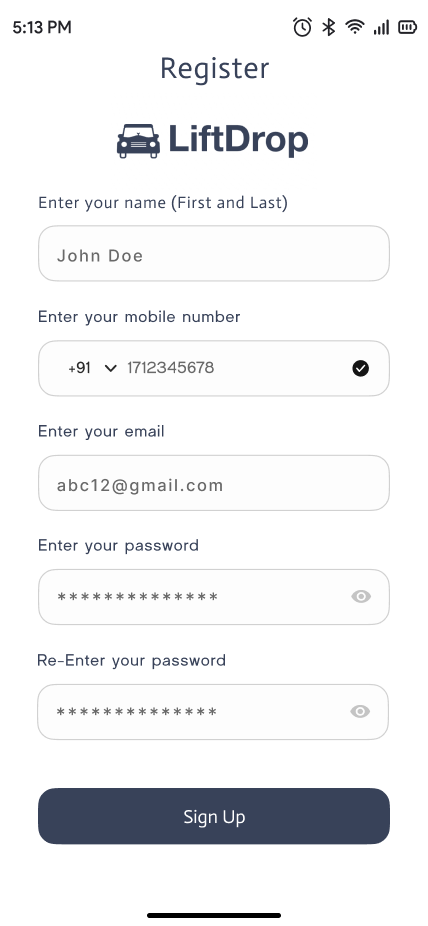
\includegraphics[width=\textwidth]{images/registration.png}
        \caption{User registration screen}
        \label{fig:registration}
    \end{subfigure}
    \hfill
    \begin{subfigure}[b]{0.44\textwidth}
        \centering
        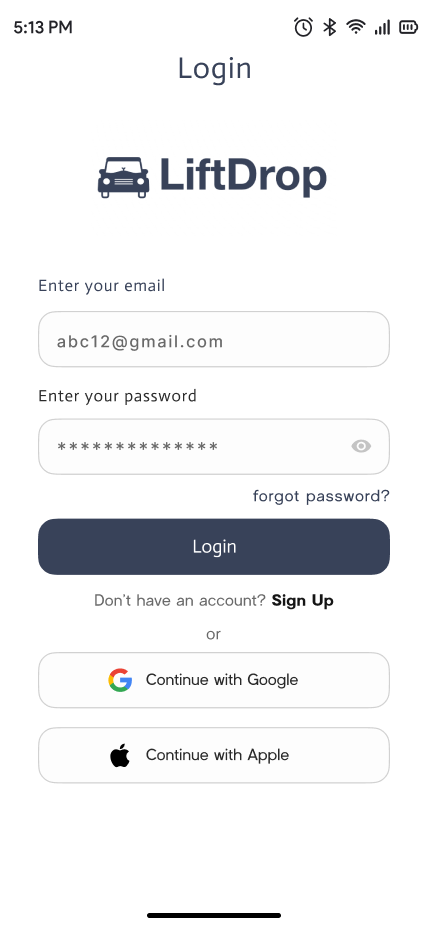
\includegraphics[width=\textwidth]{images/login.png}
        \caption{User login screen}
        \label{fig:login}
    \end{subfigure}
    \caption{Authentication flow screens for LiftDrop}
    \label{fig:auth_flow}
\end{figure}

\textbf{Registration Screen (\ref{fig:registration}):}  
Allows new users to create an account by entering essential information such as name, email, and password. This screen initiates access to the LiftDrop platform.

\textbf{Login Screen (\ref{fig:login}):}  
Enables users to securely log in using their credentials. The layout emphasizes simplicity and quick access.


\subsubsection{Courier Flow}

These screens illustrate the courier's working states, from availability to delivery.

\begin{figure}[H]
    \centering
    \begin{subfigure}[b]{0.48\textwidth}
        \centering
        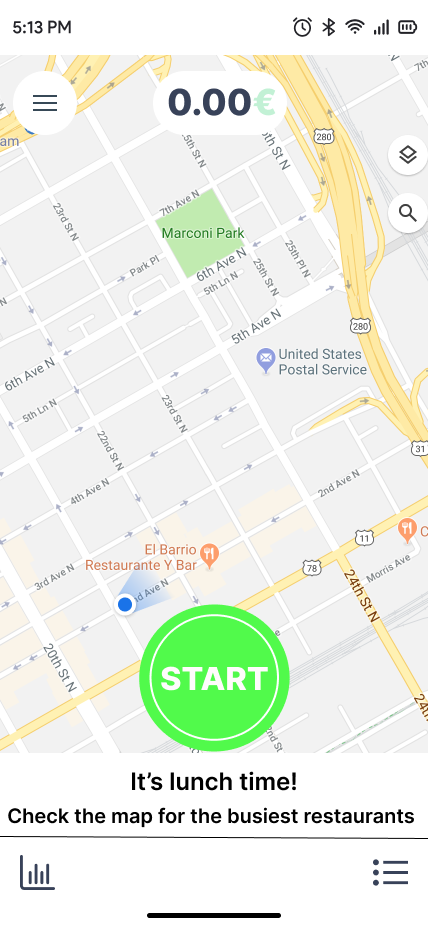
\includegraphics[width=\textwidth]{images/go_screen.png}
        \caption{Active status screen while courier is idle}
        \label{fig:go_screen}
    \end{subfigure}
    \hfill
    \begin{subfigure}[b]{0.48\textwidth}
        \centering
        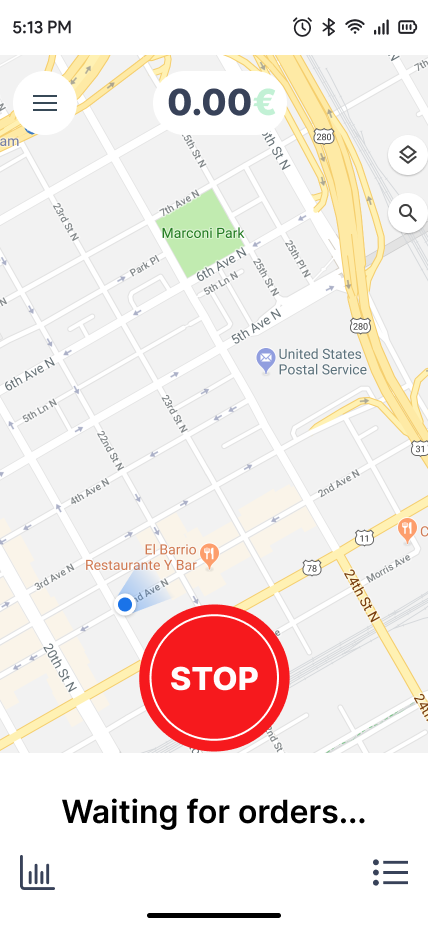
\includegraphics[width=\textwidth]{images/waiting_screen.png}
        \caption{Waiting screen during order availability check}
        \label{fig:waiting_screen}
    \end{subfigure}
    \caption{Courier status screens showing different working states}
    \label{fig:courier_status1}
\end{figure}

\textbf{Go Screen (\ref{fig:go_screen}):}  
Screen before the courier starts waiting for orders. A central status toggle makes it easy to go online or offline.

\textbf{Waiting Screen (\ref{fig:waiting_screen}):}  
Displays a waiting state while the system checks for nearby delivery requests. It reassures the user that the system is searching in the background.

\begin{figure}[H]
    \centering
    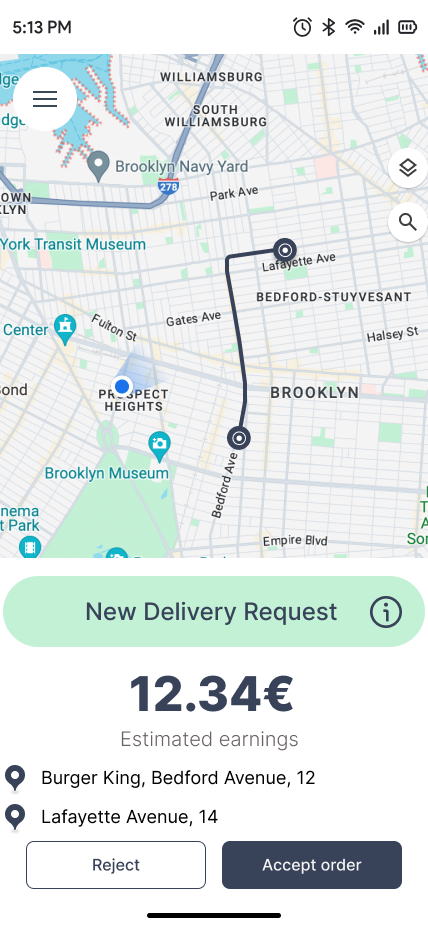
\includegraphics[width=0.6\textwidth]{images/delivery_request.png}
    \caption{New delivery request notification with order details and action buttons}
    \label{fig:delivery_request}
\end{figure}

\textbf{Delivery Request Notification (\ref{fig:delivery_request}):}  
Shows an incoming delivery request with pickup and drop-off addresses, estimated distance, and action buttons to accept or decline. It’s designed for quick decision-making and clarity.

\begin{figure}[H]
    \centering
    \begin{subfigure}[b]{0.48\textwidth}
        \centering
        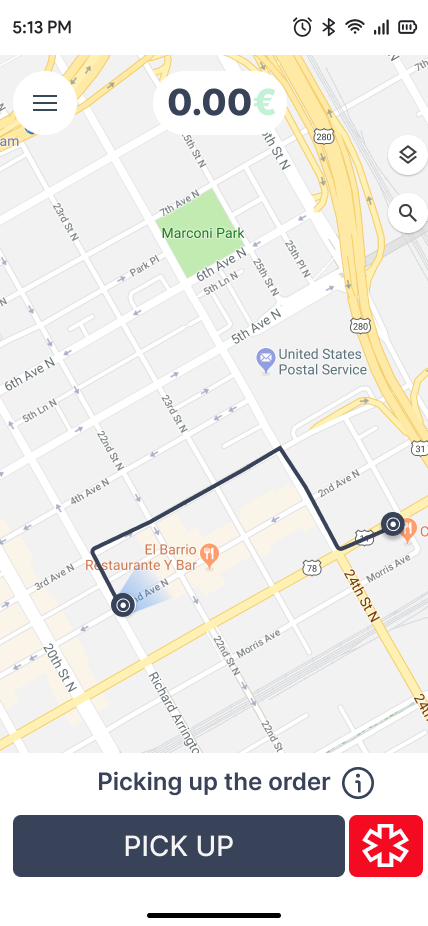
\includegraphics[width=\textwidth]{images/pickup_order_screen.png}
        \caption{Pickup Confirmation Screen}
        \label{fig:pickup_order}
    \end{subfigure}
    \hfill
    \begin{subfigure}[b]{0.48\textwidth}
        \centering
        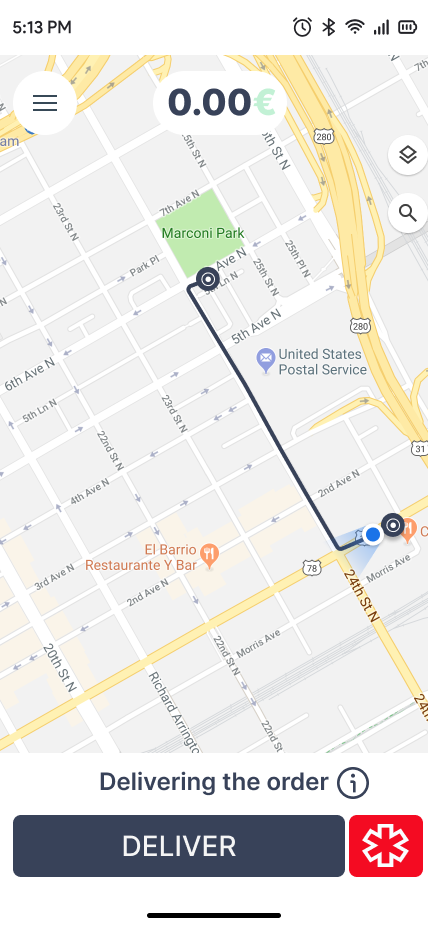
\includegraphics[width=\textwidth]{images/deliver_order_screen.png}
        \caption{Delivery Confirmation Screen}
        \label{fig:deliver_order}
    \end{subfigure}
    \caption{Courier delivery journey screens during different phases of the delivery}
    \label{fig:courier_journey}
\end{figure}

\textbf{Pickup Screen (\ref{fig:pickup_order}):}  
Provides order pickup instructions and customer location. It includes a confirmation action once the parcel is collected.

\textbf{Delivery Screen (\ref{fig:deliver_order}):}  
Guides the courier to the drop-off location. Includes proof-of-delivery options like signature or photo, depending on the order.


\subsection{System Architecture and Data Model}

This section presents different architectural perspectives of the LiftDrop system, including component-level interactions and data model relationships. Each view emphasizes a specific aspect of the system's behavior, from geolocation handling to user roles and delivery lifecycle.

\subsubsection{High-Level System Architecture}

Figure~\ref{fig:high-level-Overview} illustrates the top-level architecture of the LiftDrop platform. It shows how the Android mobile application communicates with backend services responsible for order management, user interaction, real-time communication, and location processing.

\vspace{8mm}

\begin{figure}[H]
    \centering
    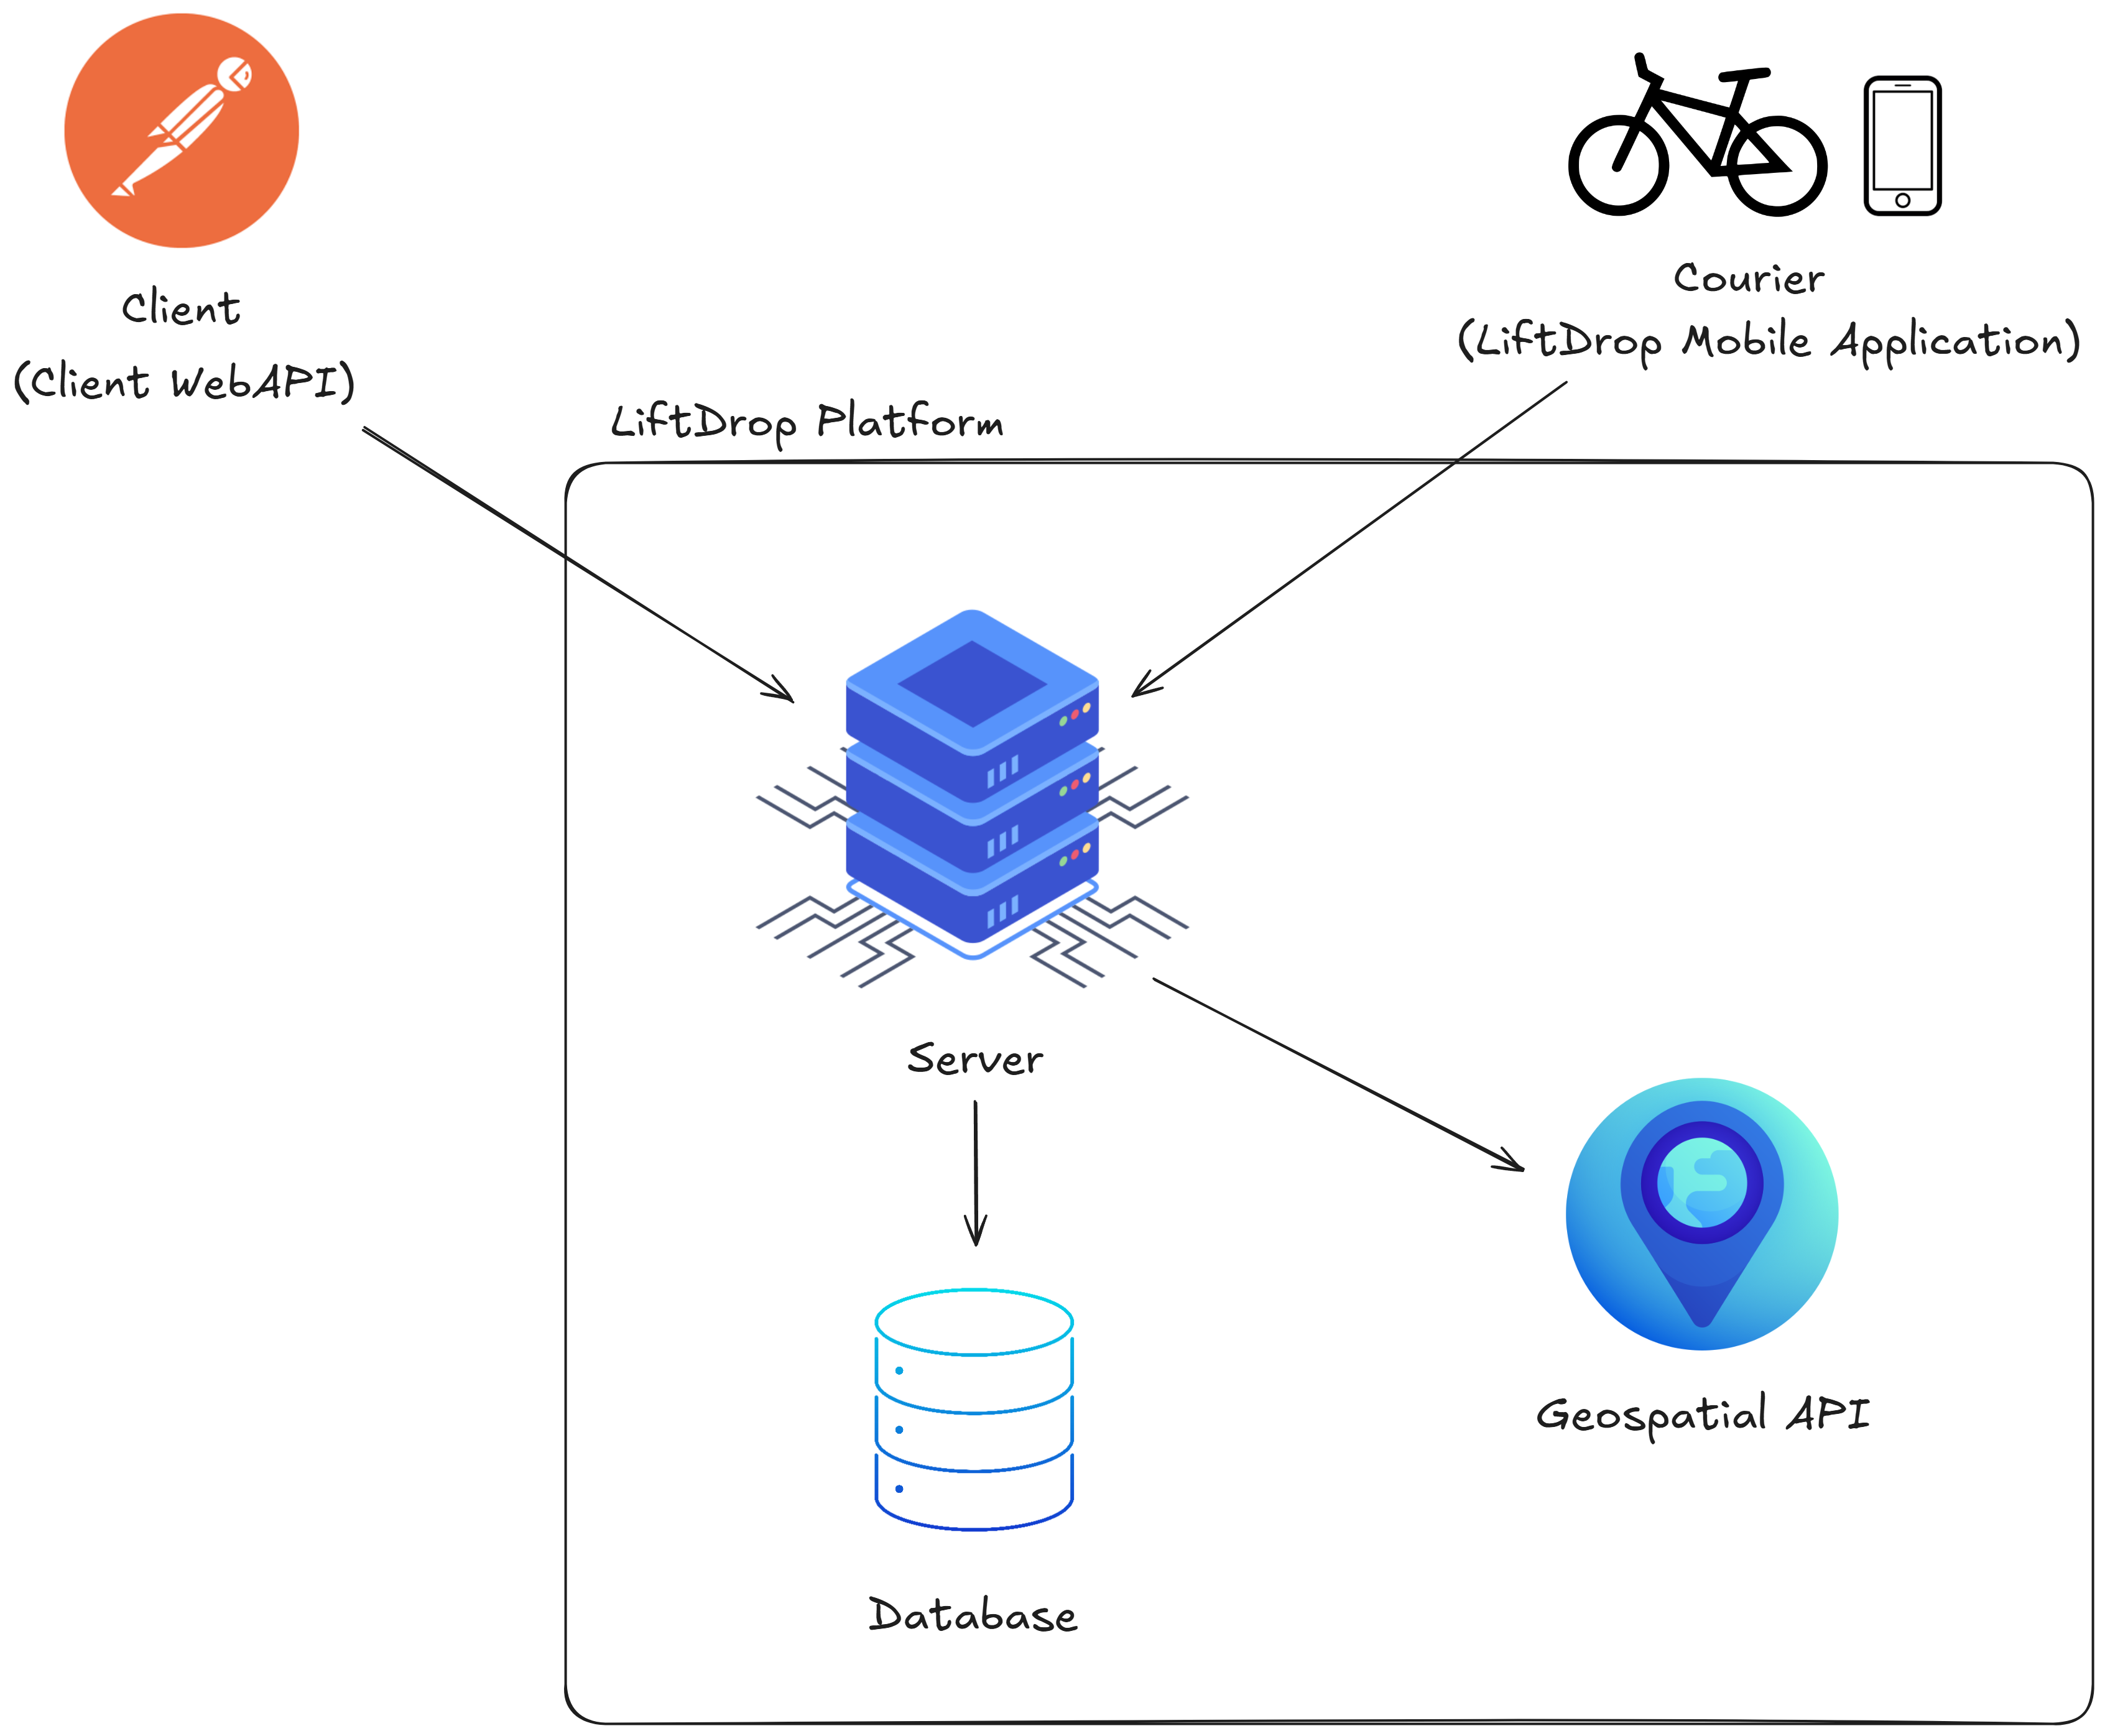
\includegraphics[width=0.82\textwidth]{images/LiftDrop_High_level_view.png}
    \caption{High-level overview of the LiftDrop system architecture}
    \label{fig:high-level-Overview}
\end{figure}

\newpage

\subsubsection{Location Model Overview}

This view isolates the system's handling of geospatial information. The \texttt{Location} class acts as a base abstraction for different types of spots used during a delivery. Specialized entities like \texttt{PickupSpot} and \texttt{DropOffSpot} inherit from \texttt{Location}, allowing consistent treatment of position data. A pickup spot can contain multiple \texttt{Item} entries, each identified by a unique designation.

\begin{figure}[H]
    \centering
    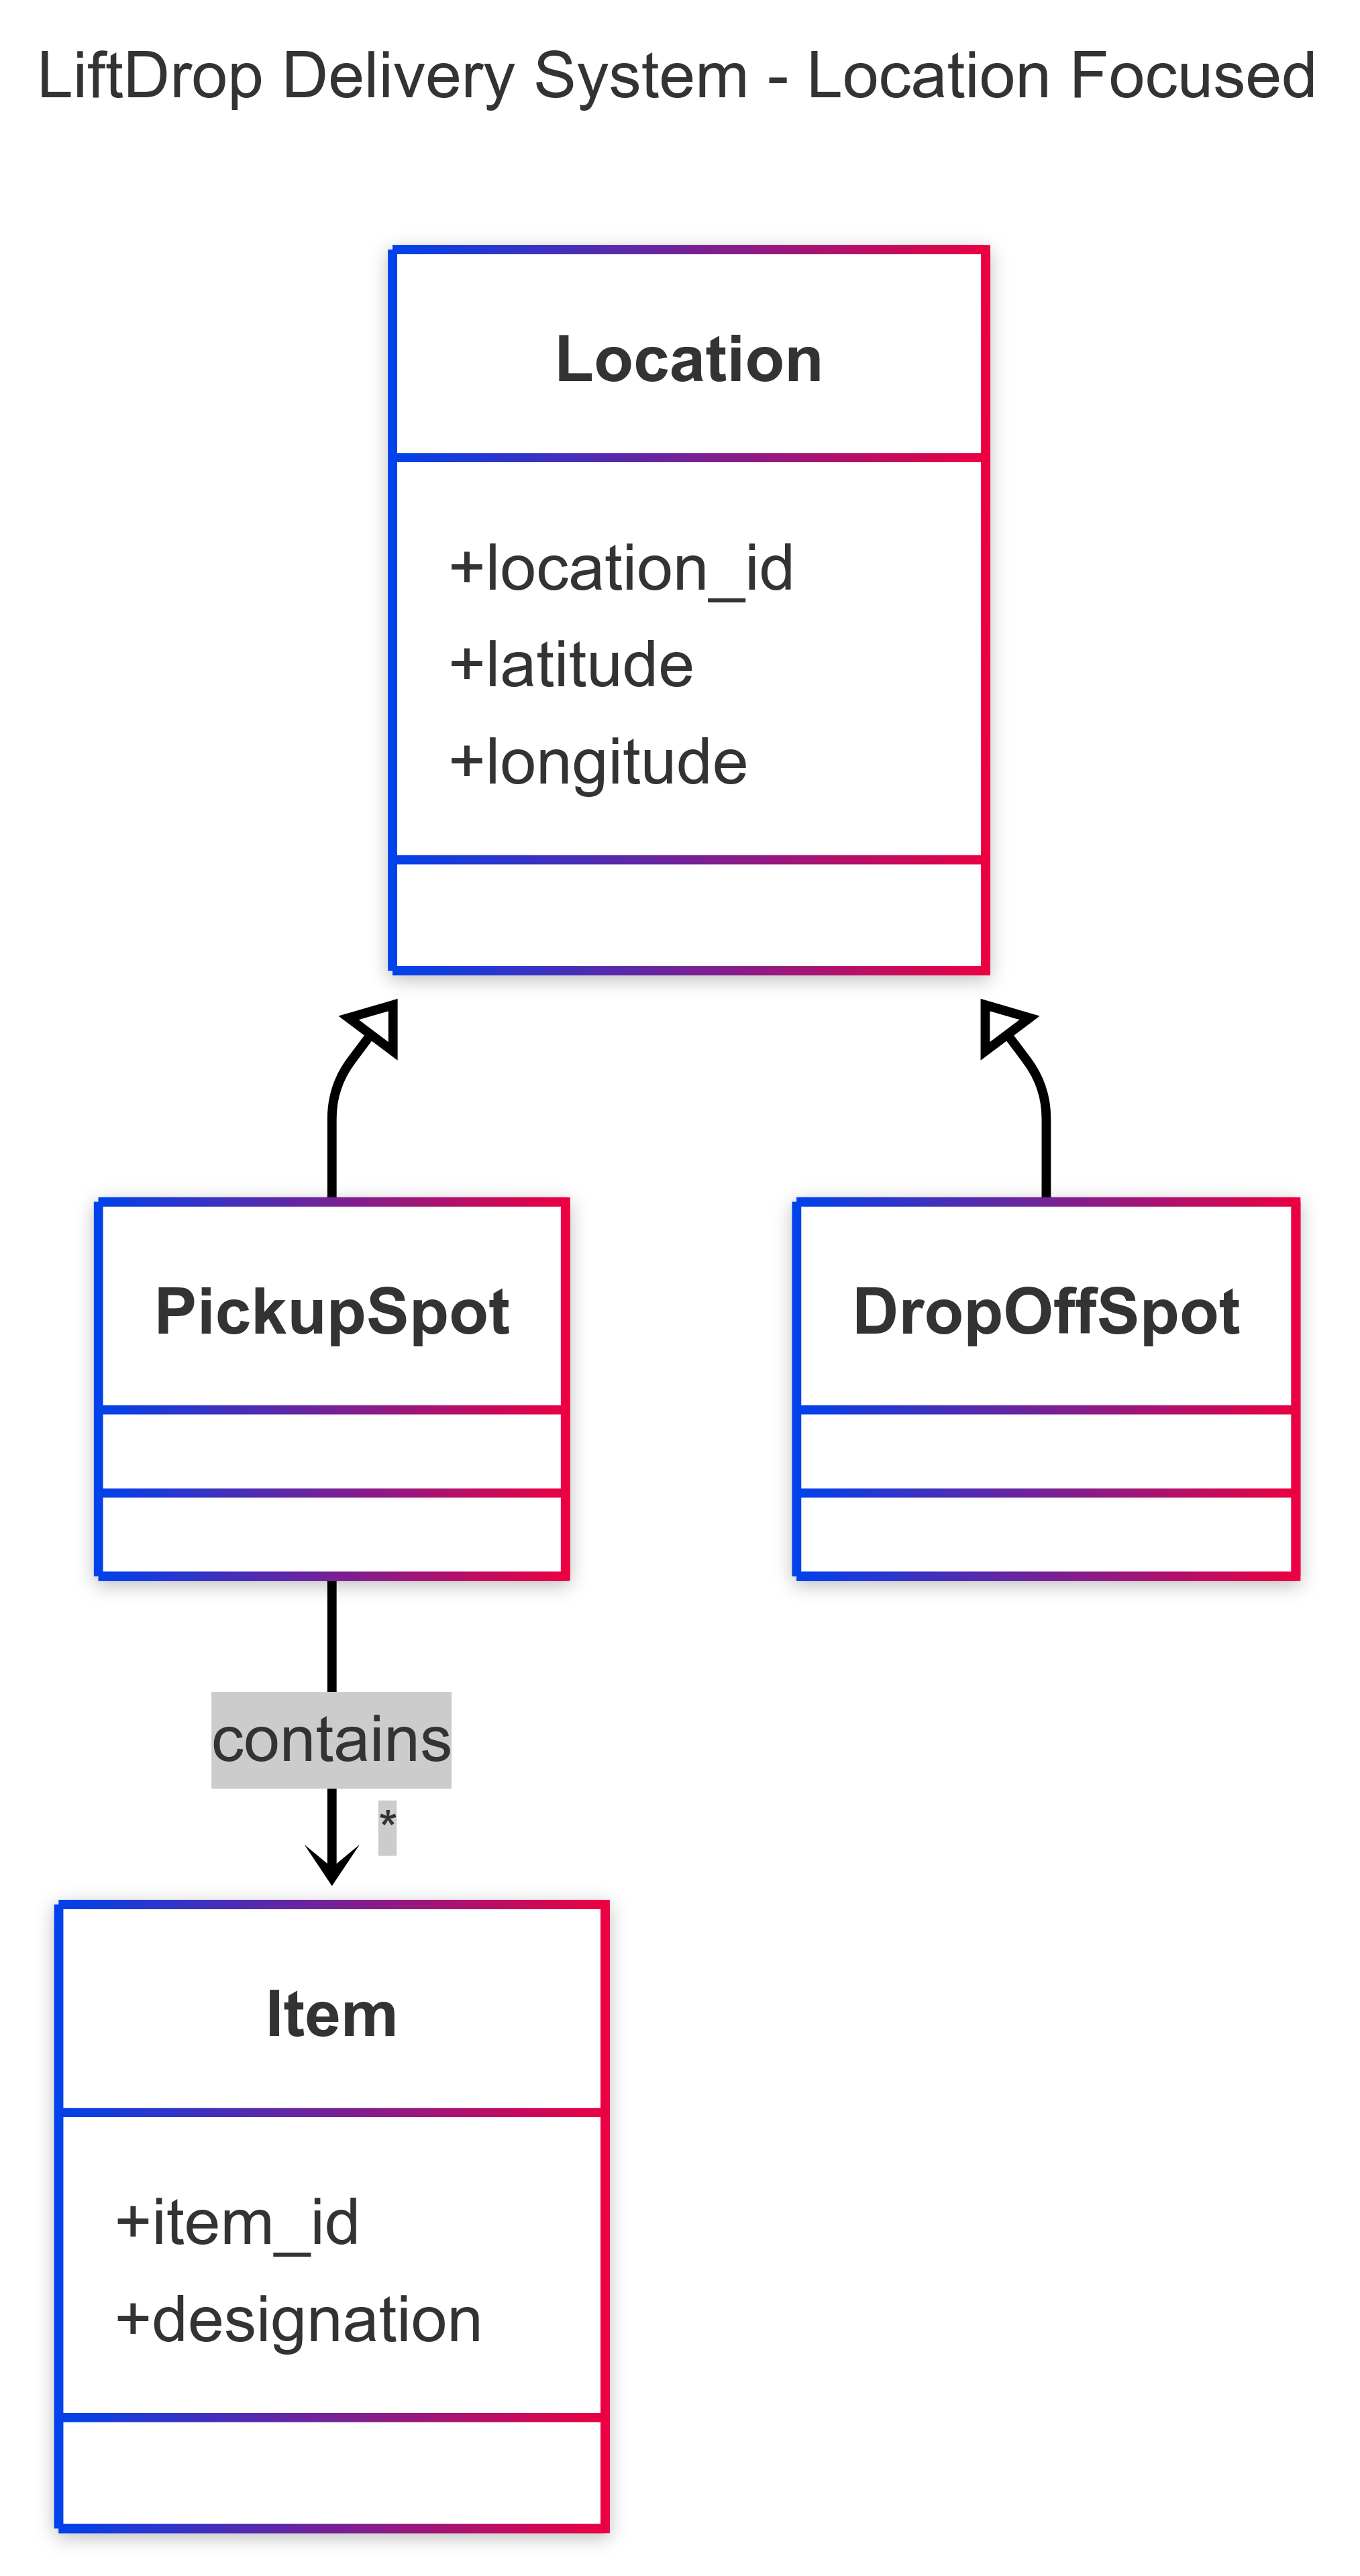
\includegraphics[width=0.44\textwidth]{images/LocationDiagram.png}
    \caption{Location Model Structure}
\end{figure}

\newpage

\subsubsection{User Role and Interaction Model}

This simplified diagram captures user roles and their interaction with delivery workflows. A \texttt{Client} can place multiple \texttt{Request}s, and a \texttt{Courier} can fulfill many of them. Each request is linked to a corresponding \texttt{Delivery}, forming a one-to-one mapping between a request and its fulfillment.
  
\begin{figure}[H]
    \centering
    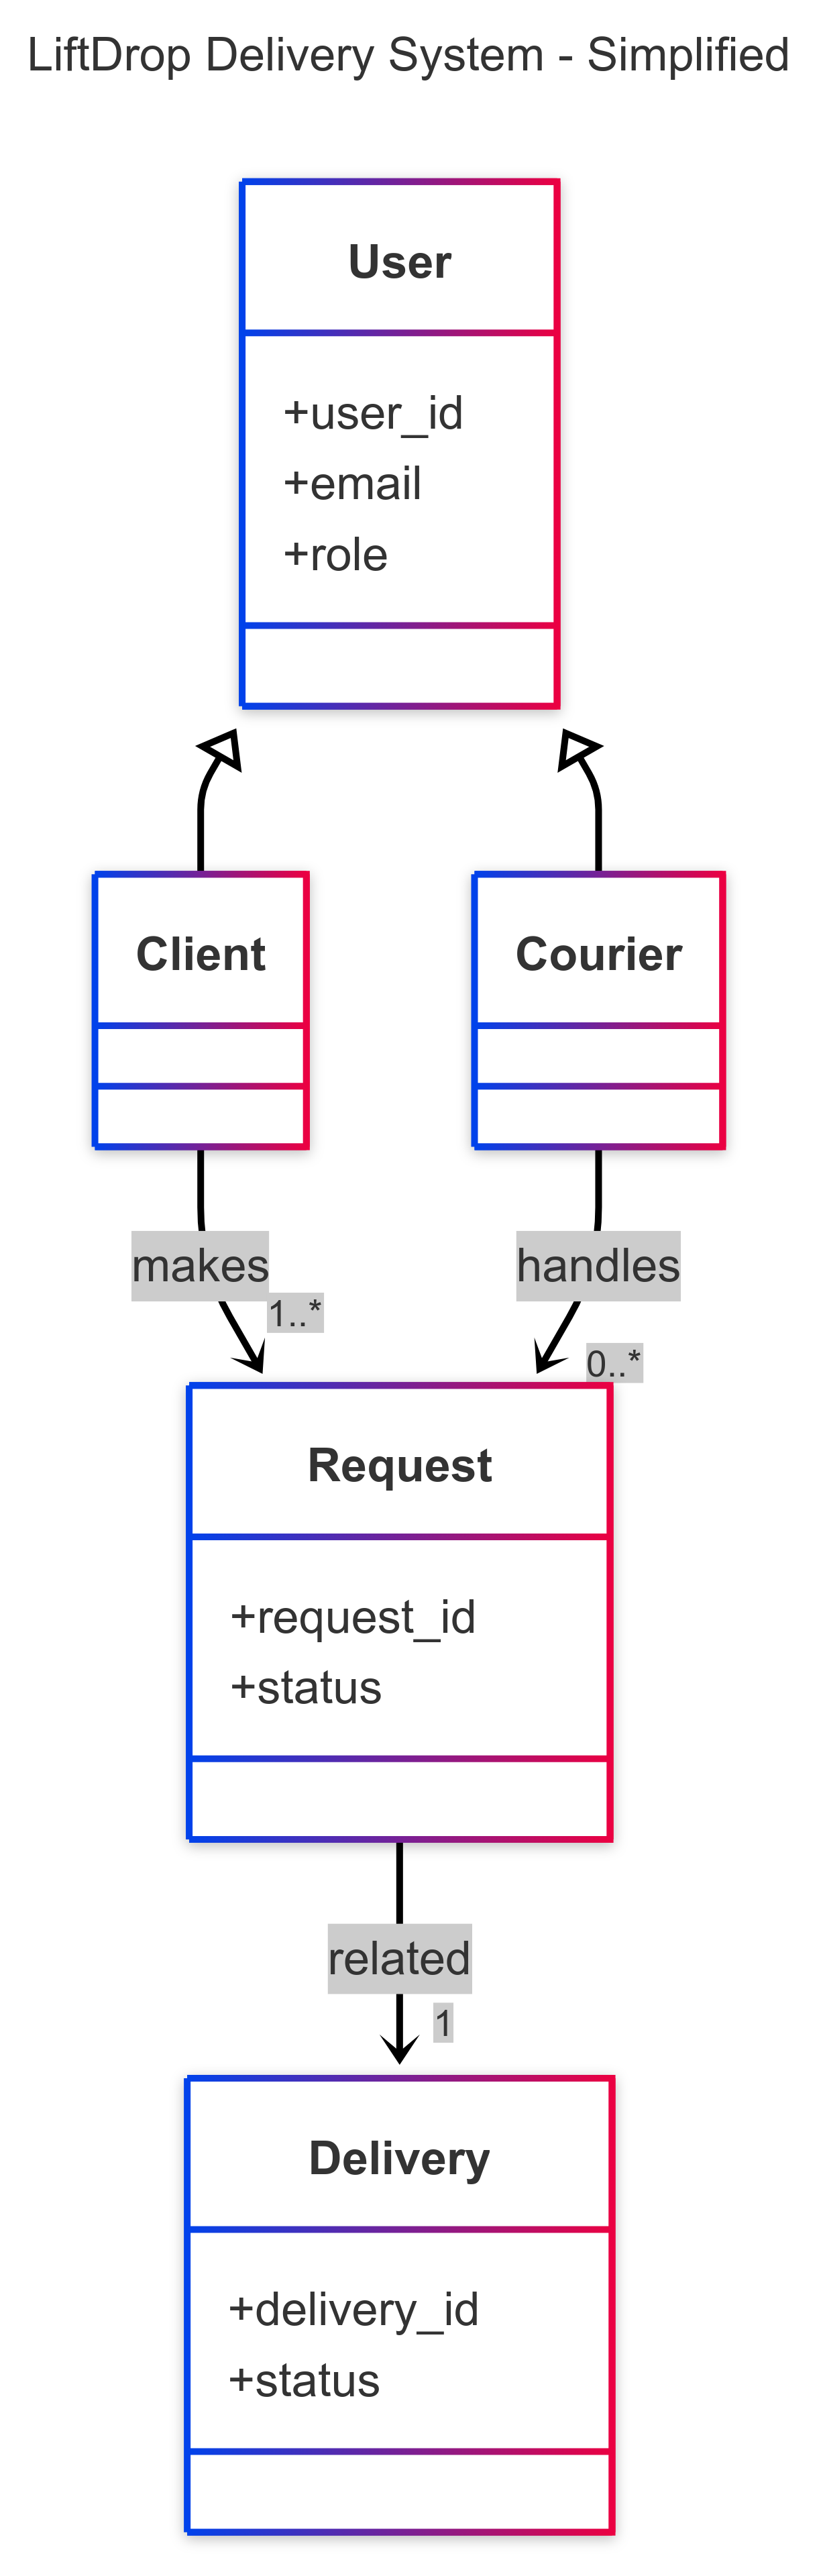
\includegraphics[width=0.40\textwidth]{images/UserClientCourierDiagram.png}
    \caption{User and Role Relationships}
\end{figure}

\subsubsection{Request and Delivery Lifecycle View}

This view focuses on how a request progresses through the system. Each \texttt{Request} includes additional metadata encapsulated in a \texttt{RequestDetails} object and is associated with a single \texttt{Delivery}. This structure supports clear traceability and separation of concerns between request creation and execution.

\begin{figure}[H]
    \centering
    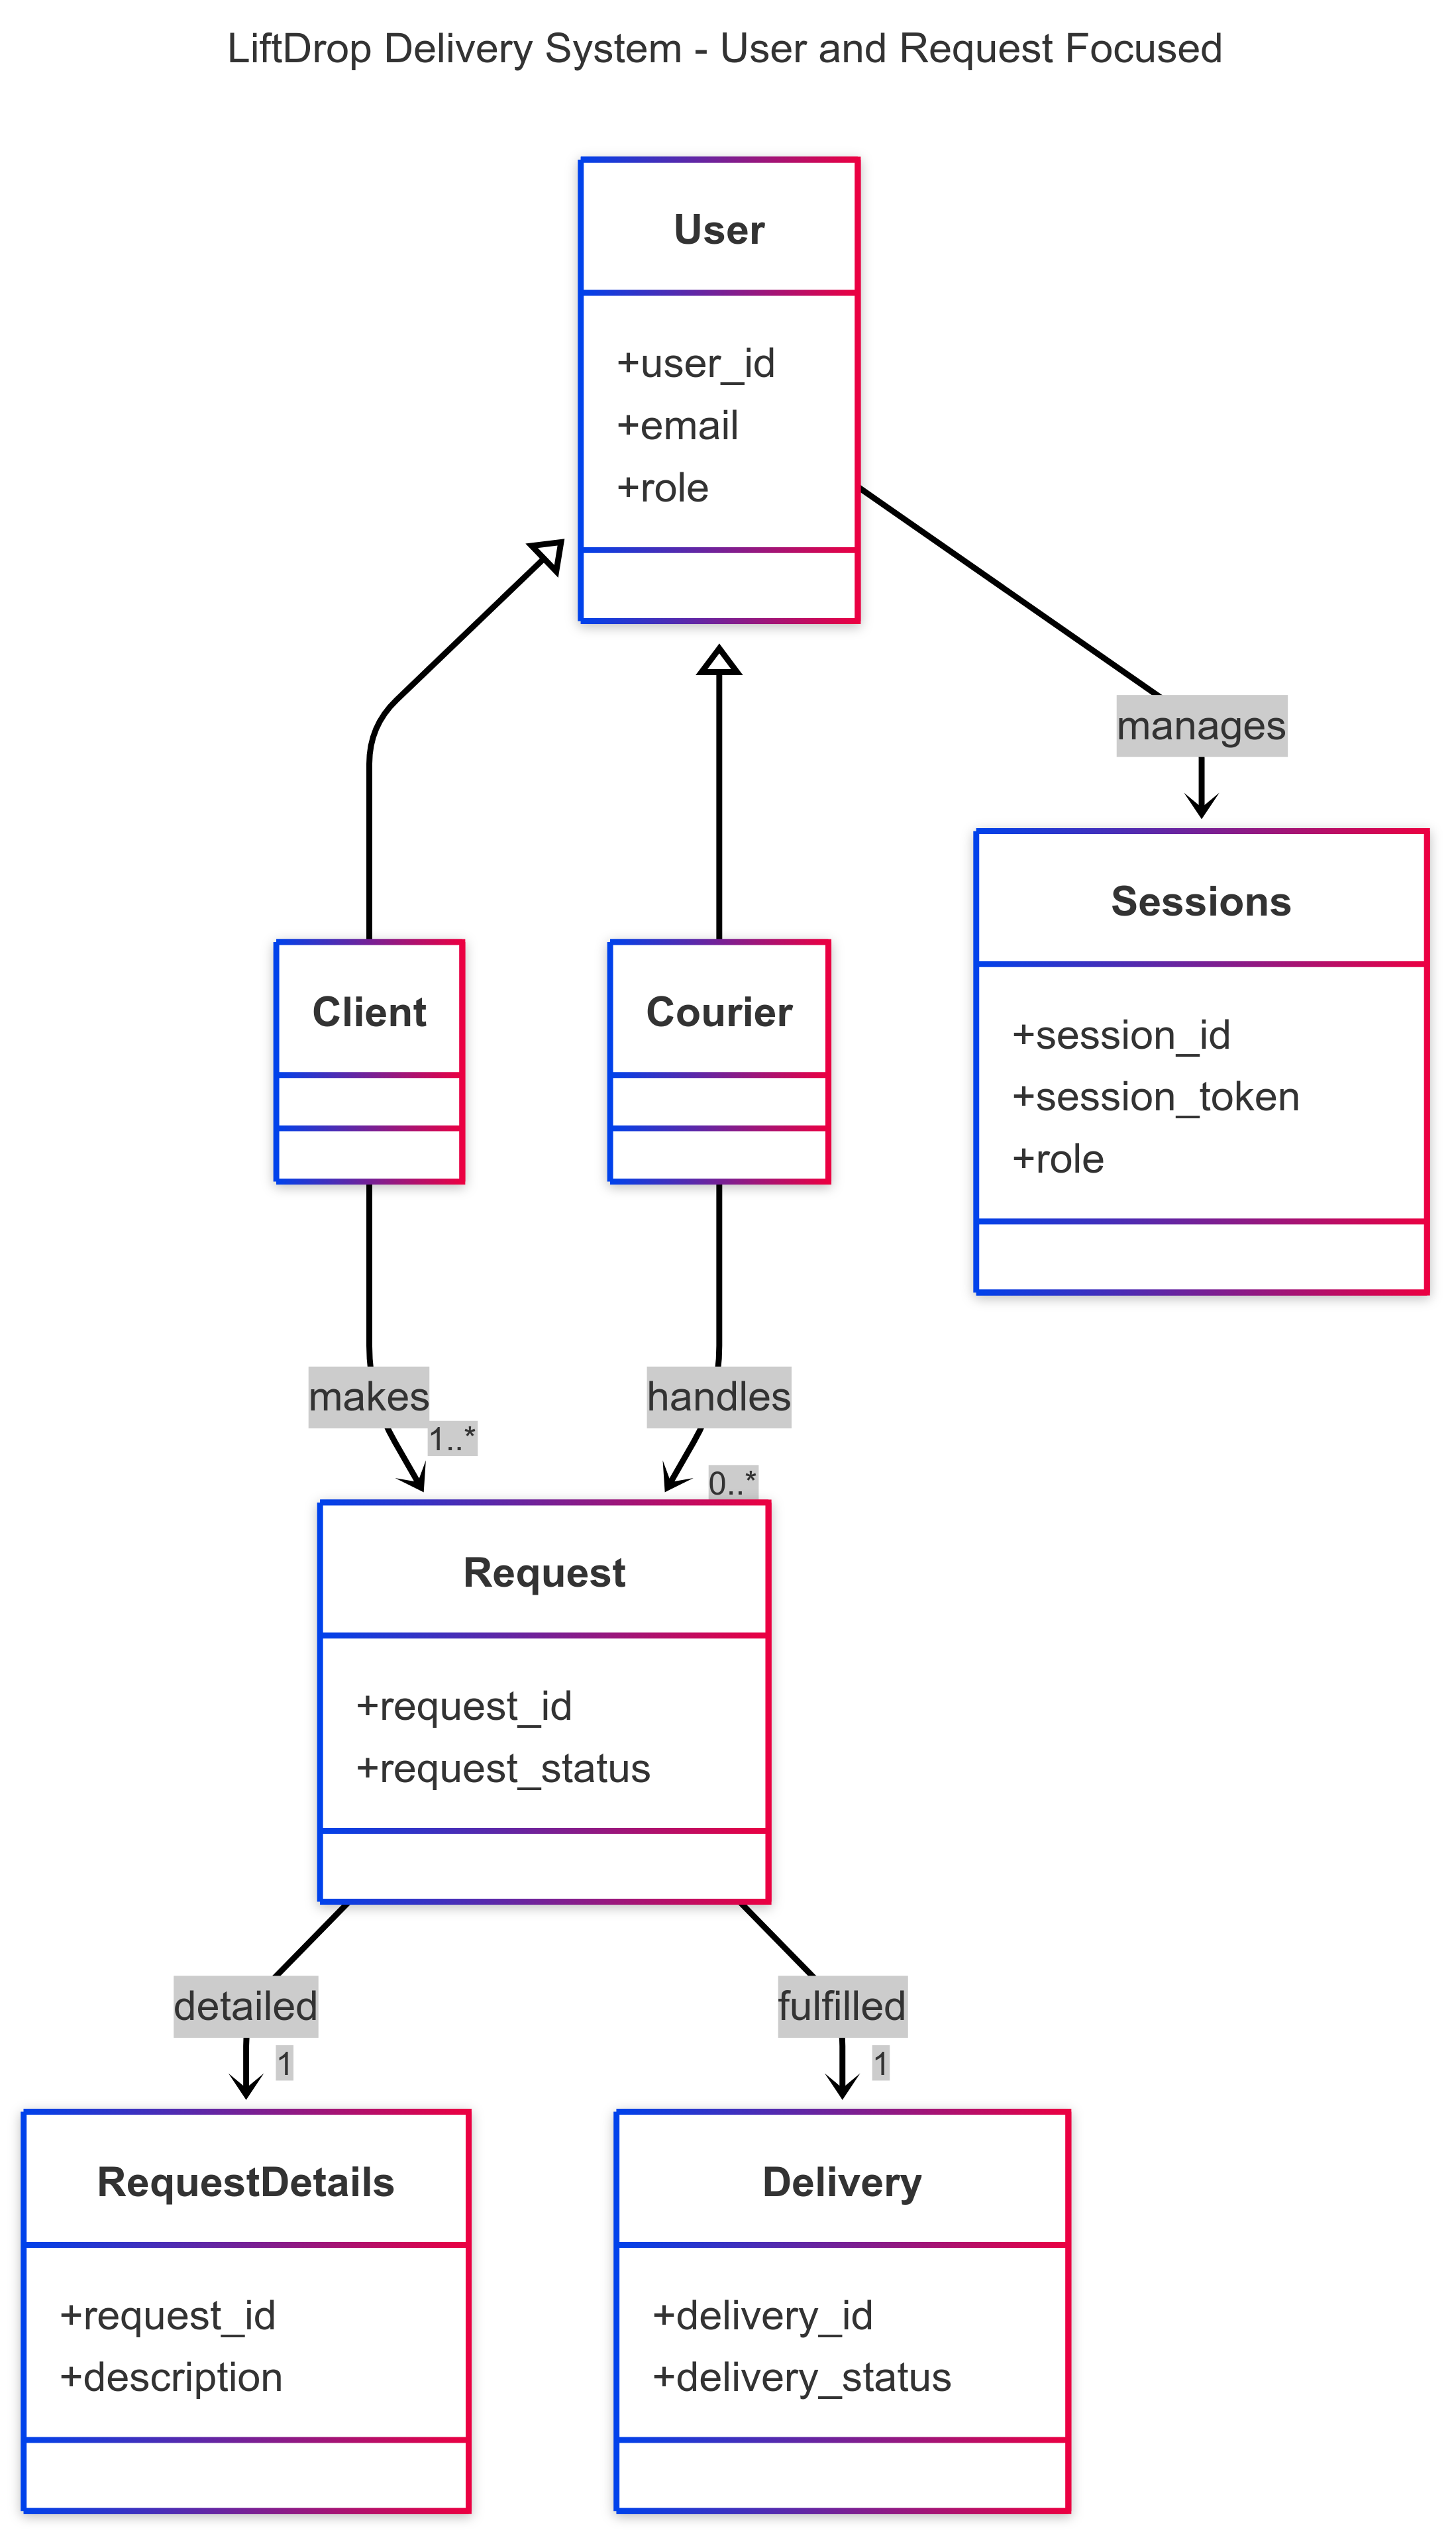
\includegraphics[width=0.44\textwidth]{images/UserSessions.png}
    \caption{Request and Fulfillment Architecture}
\end{figure}

\newpage

\subsubsection{Comprehensive System Model}

The complete data model integrates all key domain entities: \texttt{User}, \texttt{Address}, \texttt{Location}, \texttt{Item}, \texttt{Request}, \texttt{Delivery}, and \texttt{Session}. It captures how users interact with the system, how orders are structured and routed, and how real-time delivery coordination is maintained through geolocation and session-aware tracking.

\begin{figure}[H]
    \centering
    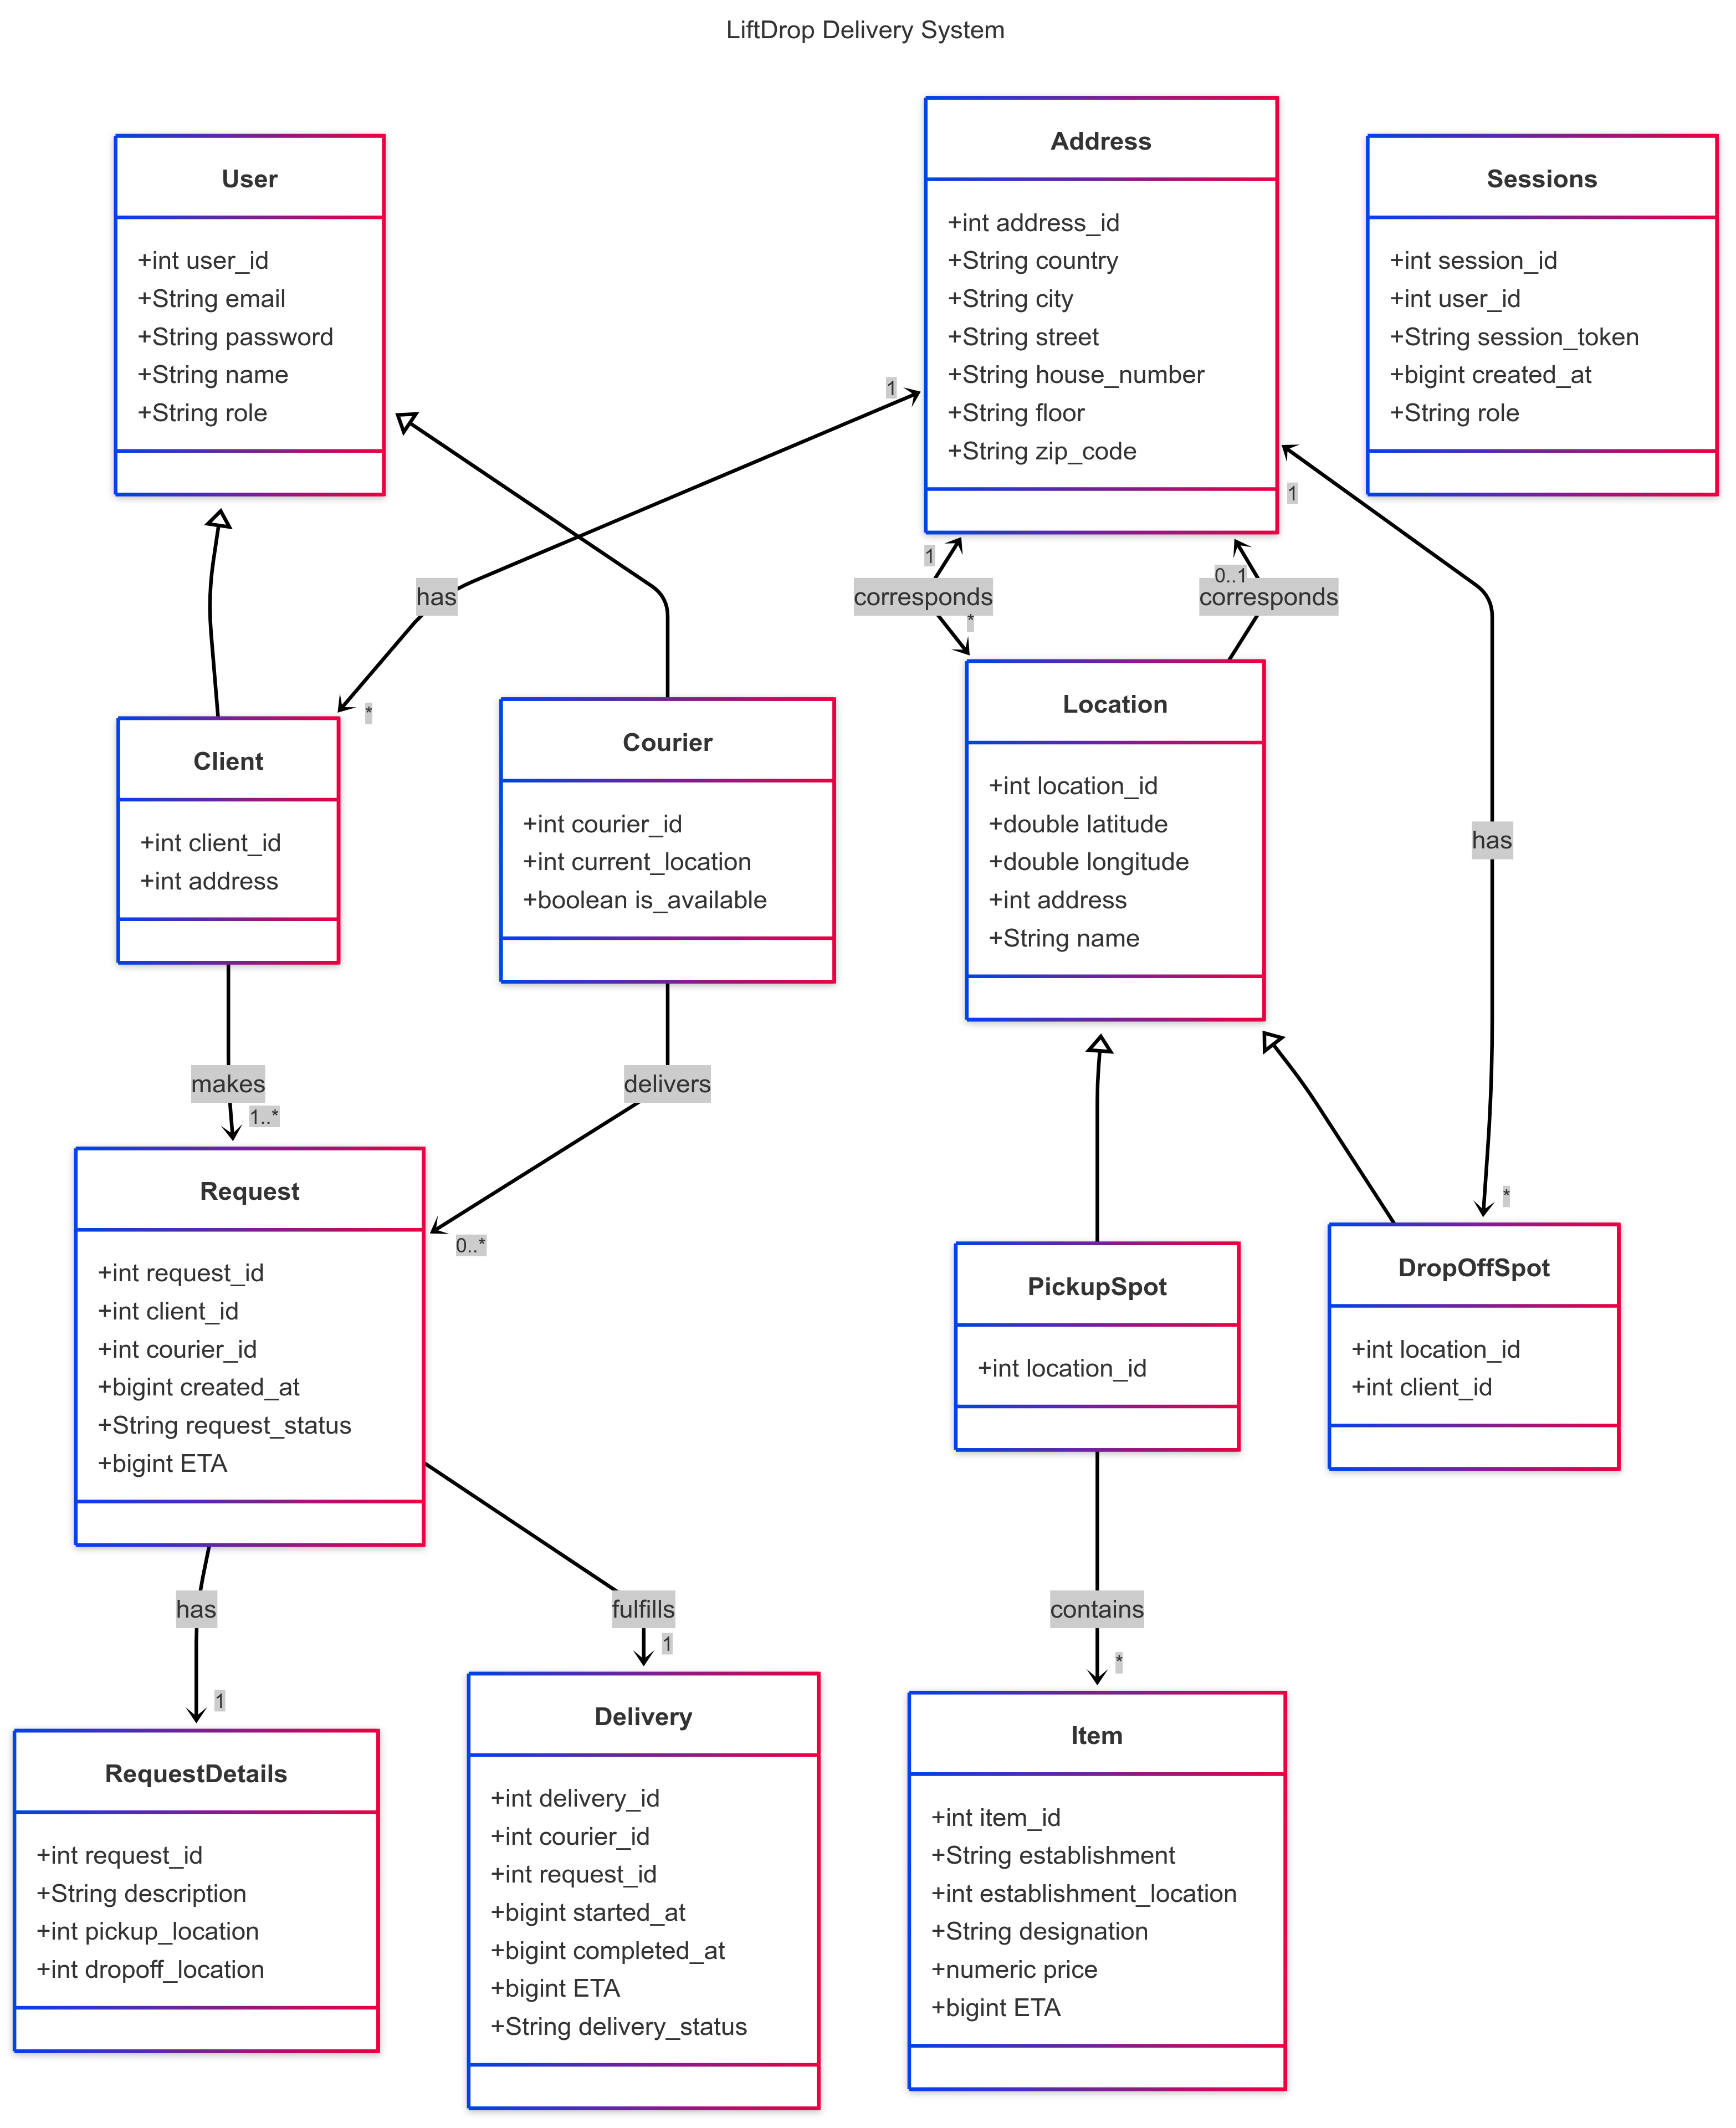
\includegraphics[width=0.8\textwidth]{images/FullDiagram.png}
    \caption{Full System Data Model}
\end{figure}


\end{document}
